\documentclass{SKP-beamer}

% --------------------------------------------------- %
%                  Presentation info	              %
% --------------------------------------------------- %
\title[Cloud Computing]{CLOUD COMPUTING}
\subtitle{Cloud Computing - Overview}
\author{PROF.SOUMYA K.GHOSH}
\institute[SIT]{
  SILICON INSTITUTE OF TECHNOLOGY\\
  SAMBALPUR
}
\date{\today}
\logo{
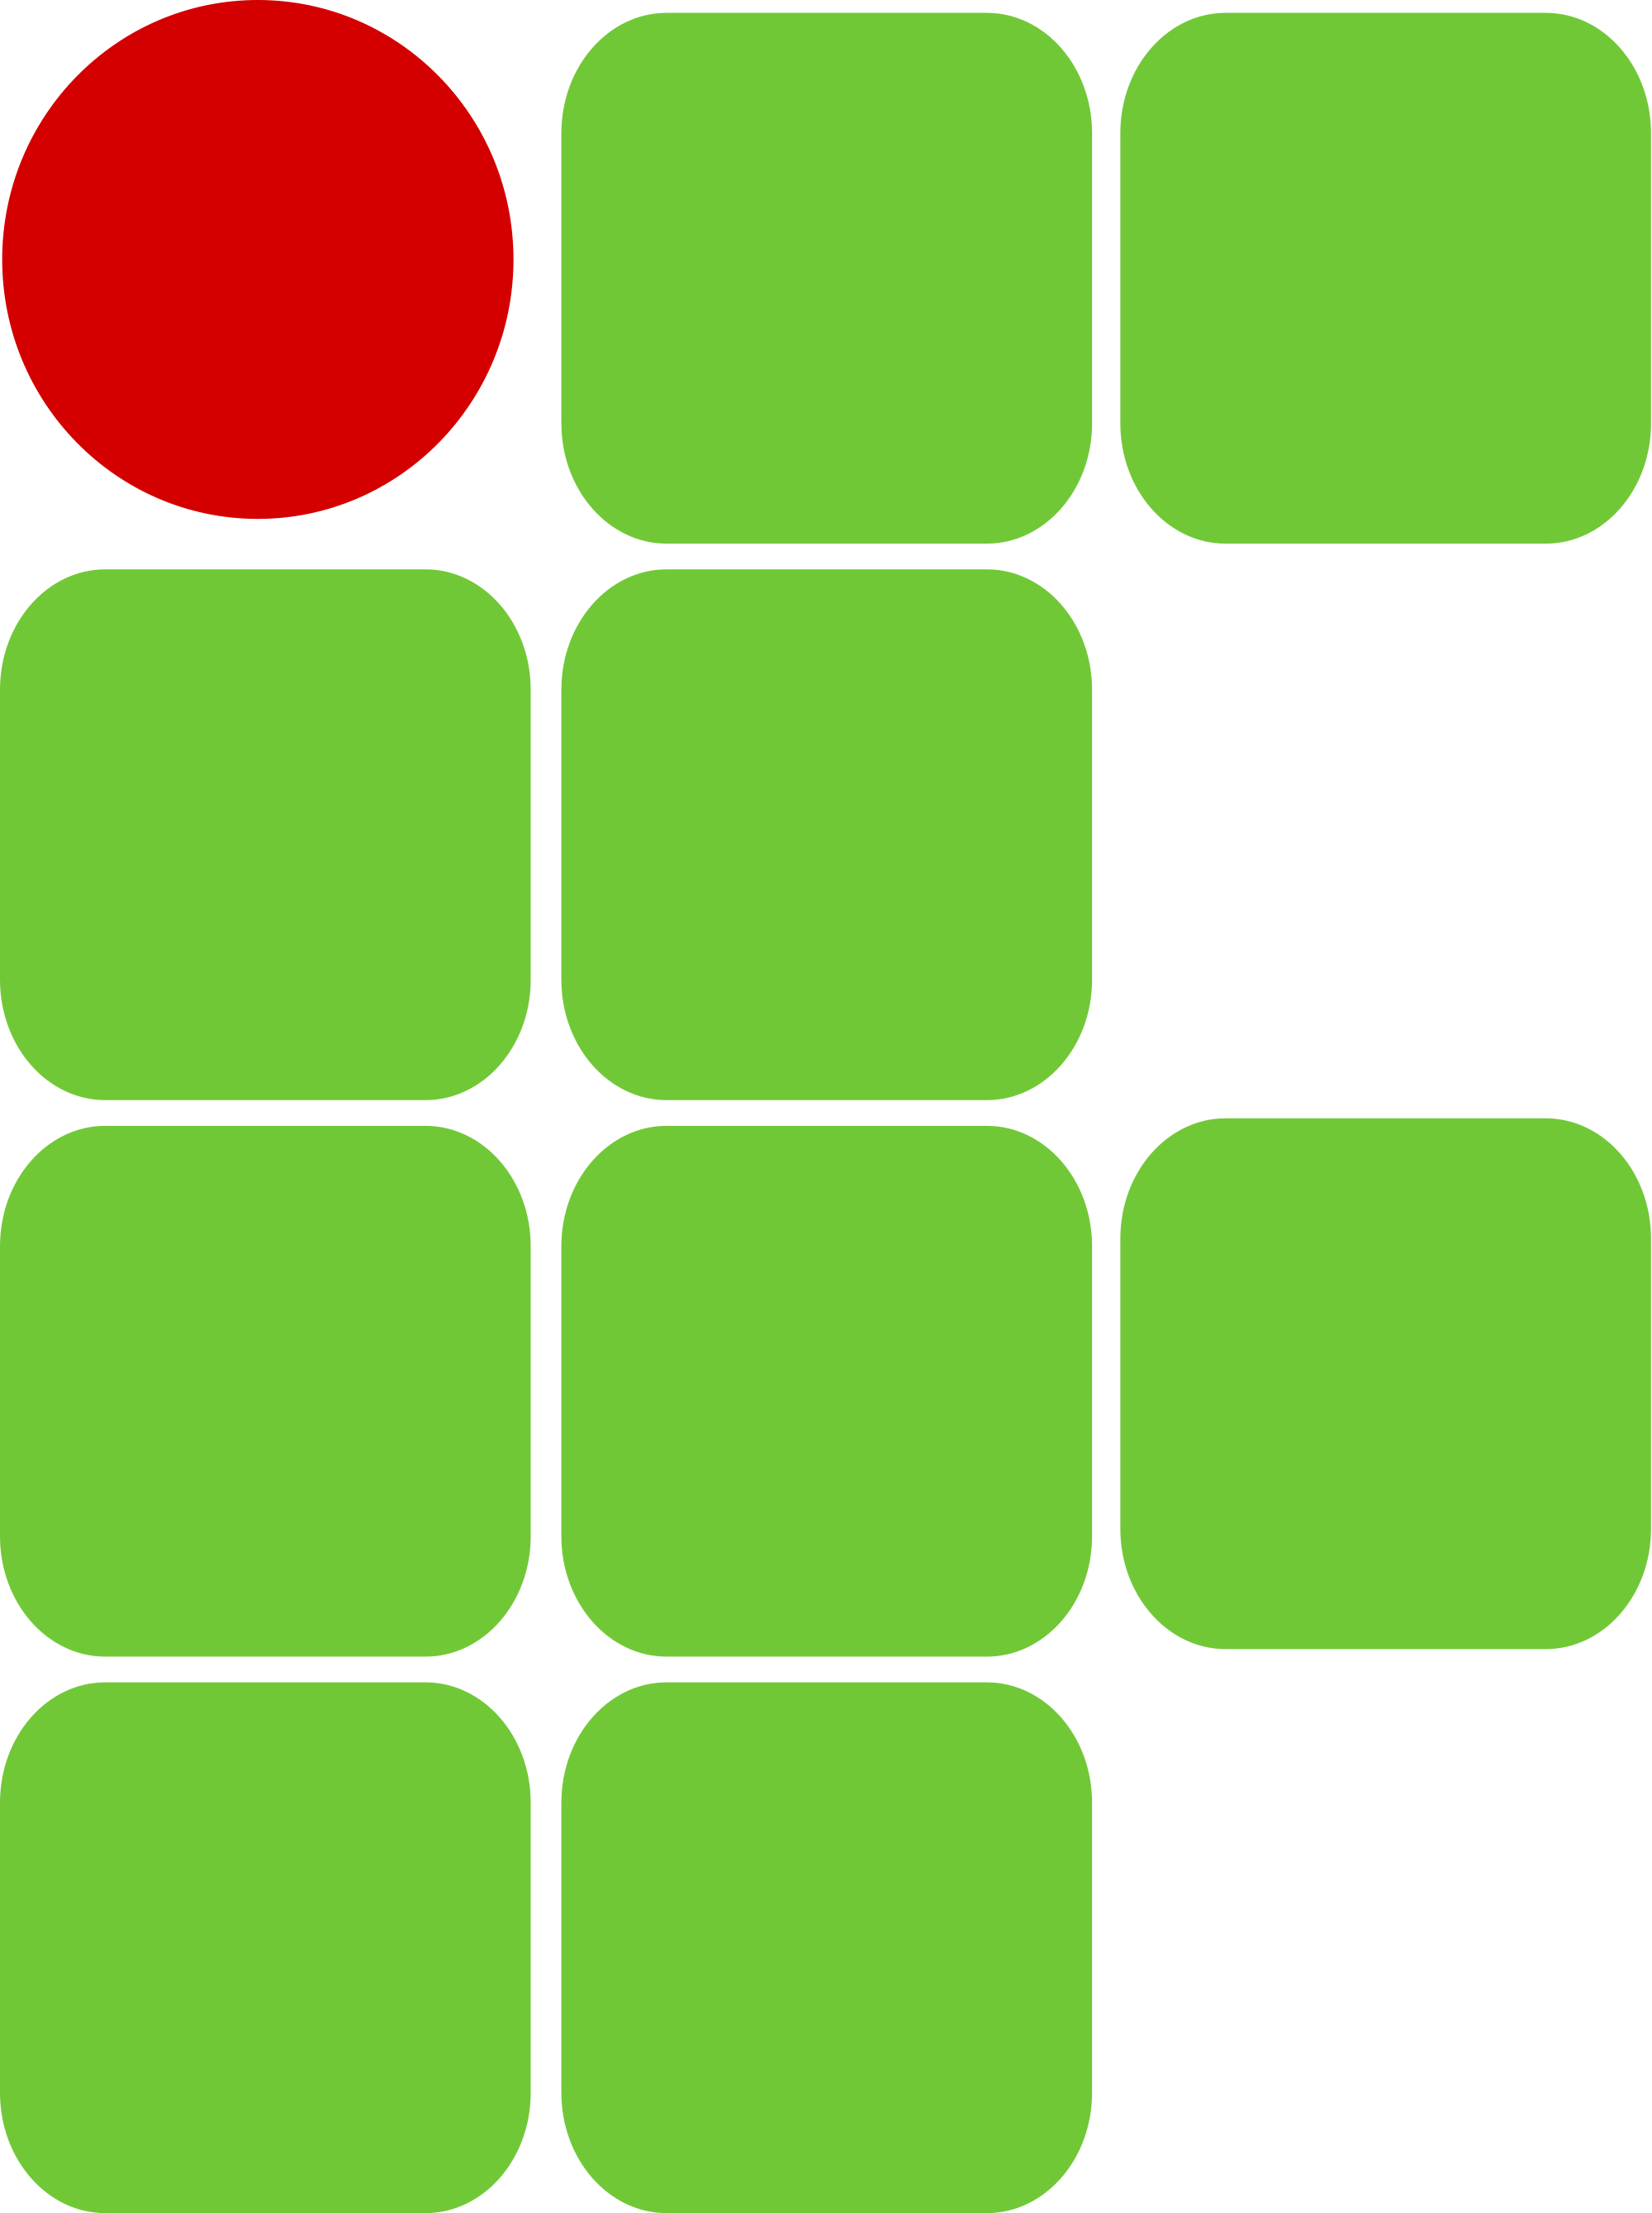
\includegraphics[scale=0.008]{images/logo.png}
}
\subject{Presentation subject} % metadata

% --------------------------------------------------- %
%                    Title + Schedule                 %
% --------------------------------------------------- %

\begin{document}

\begin{frame}
  \titlepage
\end{frame}

\begin{frame}{Introduction}
  The ACM Computing Curricula 2005 defined "computing" as
  
  "In a general way, we can define computing to mean any goal-oriented activity  requiring,  benefiting  from,  or  creating  computers.  Thus, computing includes designing and building hardware and software systems for a wide range of purposes; processing, structuring, and managing various kinds of information; doing scientific studies using computers; making computer systems behave intelligently; creating and  using  communications  and  entertainment  media;  finding  and gathering information relevant to any particular purpose, and so on. The list is virtually endless, and the possibilities are vast."
  
\end{frame}



\begin{frame}{Cloud Computing Course - Overview}
	\begin{itemize}
		\item  Introduction to Cloud Computing
		\begin{itemize}
			\item  Overview of Computing
			\item Cloud Computing (NIST Model)
			\item Properties, Characteristics & Disadvantages
			\item Role of Open Standards
			
		\end{itemize}
		\item Cloud Computing Architecture
			\begin{itemize}
			\item  Cloud computing stack
            \item  Service Models (XaaS)
		        \begin{itemize}
		        	\item  Infrastructure as a Service(IaaS)
		        	\item  Platform as a Service(PaaS)
		        	\item Software as a Service(SaaS)
		        \end{itemize}
			\item  Deployment Models
	    	\end{itemize}
		\item Service Management in Cloud Computing
		        	\begin{itemize}
		        	\item  Service Level Agreements(SLAs)
		        	\item  Cloud Economics
		        	 \end{itemize}
		 \item Resource Management in Cloud 
		 Computing
		 
	\end{itemize}
	
\end{frame}


\begin{frame}{Cloud Computing Course (contd.)}
	\begin{itemize}
		\item  Data Management in Cloud Computing
		\begin{itemize}
			\item  Looking at Data, Scalability & Cloud Services
			\item Database & Data Stores in Cloud
			\item Large Scale Data Processing
		\end{itemize}
		\item Cloud Security
		\begin{itemize}
			\item Infrastructure Security
			\item Data security and Storage
			\item Identity and Access Management
			\item Access Control, Trust, Reputation, Risk
		\end{itemize}
		\item Case Study on Open Source and Commercial Clouds, Cloud Simulator
		\item Research trend in Cloud Computing, Fog Computing
		
		
	\end{itemize}
	
\end{frame}


% --------------------------------------------------- %
%                      Presentation                   %
% --------------------------------------------------- %



\begin{frame}{Trends in Computing}
		\begin{itemize}
		\item Distributed Computing
		\item Grid Computing
		\item Cluster Computing
		\item Utility Computing
		\item \textbf{Cloud Computing}
		
	\end{itemize}
\end{frame}

\section{Distributed Computing}


\begin{frame}{Centralized vs. Distributed Computing}
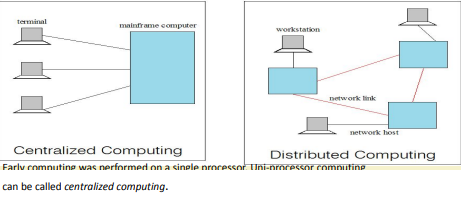
\includegraphics[scale=1.2]{1.png}
\end{frame}


\begin{frame}{Distributed Computing/System?}
	\begin{itemize}
		\item Distributed Computing
		\begin{itemize}
			\item  Field of computing science that studies distributed system
			\item Use of distributed systems to solve computational problems.		
		\end{itemize}
		\item Distributed Computing
		\begin{itemize}
			\item Wikipedia
			
			\begin{itemize}
				\item  There are several autonomous computational entities, 
				each of which has its own local memory.
				\item The entities communicate with each other by message 
				passing.		
			\end{itemize}		
			
			\item Operating System Concept
				\begin{itemize}
				\item The processors communicate with one another through various 
				communication lines, such as high-speed buses or telephone 
				lines.
				\item Each processor has its own local memory.		
			\end{itemize}
		\end{itemize}
		
		
	\end{itemize}
	
	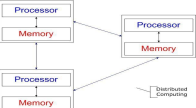
\includegraphics[scale=1.2]{2.png}
	
\end{frame}


\begin{frame}{Example Distributed Systems}
	\begin{itemize}
		\item Internet
		\item ATM(bank) machines
		\item Intranets/Workgroups
		\item Computing landscape will soon consist of 
		ubiquitous network-connected devices
		
		
	\end{itemize}
\end{frame}


\begin{frame}{Computers in a Distributed System}
	\begin{itemize}
		\item Workstations : Computers used by end-users to perform 
		computing
		\item Server Systems: Computers which provide resources and
		services
		\item Intranets/Workgroups
		\item Personal Assistance Devices: Handheld computers connected to the system via a wireless communication link.
		
	\end{itemize}
\end{frame}

\begin{frame}{Common properties of Distributed Computing}
	\begin{itemize}
		\item Fault tolerance
		\begin{itemize}
			\item  When one or some nodes fails, the whole system can still work fine except performance.
			\item Need to check the status of each node
		\end{itemize}
		\item Each node play partial role
		\begin{itemize}
			\item Each computer has only a limited, incomplete view of the system
			\item Each computer may know only one part of the input.
		\end{itemize}
		\item Resource sharing
		\begin{itemize}
			\item Each user can share the computing power and storage resource in the system with other 
			users
		\end{itemize}
		\item Load Sharing
			\begin{itemize}
			\item Dispatching several tasks to each nodes can help share loading to the whole system.
		\end{itemize}
		\item Easy to expand
		\begin{itemize}
			\item We expect to use few time when adding nodes. Hope to spend no time if possible.
		\end{itemize}
		\item Performance
		\begin{itemize}
			\item Parallel computing can be considered a subset of distributed computing.
		\end{itemize}
	\end{itemize}
	
\end{frame}


\begin{frame}{Why Distributed Computing?}
	\begin{itemize}
		\item Nature of application
		\item Performance
		
	
         	-- Computing Intensive
		\begin{itemize}
		\item The task could consume a lot of time on computing. For 
		example, Computation of Pi value using Monte Carlo simulation
	\end{itemize}
	       -- Data Intensive
	       \begin{itemize}
	       	\item The task that deals with a large amount or large size of files. For 
	       	example, Facebook, LHC(Large Hadron Collider) experimental data 
	       	processing.
	       \end{itemize}
	     \item Robustness \\
	       -- No SPOF (Single Point Of Failure)\\
	       -- Other nodes can execute the same task executed on failed 
	       node.
	       
    \end{itemize}
\end{frame}


\section{\textbf{THANK YOU!!}}

\begin{frame}
	\titlepage
\end{frame}


\begin{frame}{Why Distributed Computing?}
	\begin{itemize}
		\item Nature of application
		\item Performance
		
		
		-- Computing Intensive
		\begin{itemize}
			\item The task could consume a lot of time on computing. For 
			example, Computation of Pi value using Monte Carlo simulation
		\end{itemize}
		-- Data Intensive
		\begin{itemize}
			\item The task that deals with a large amount or large size of files. For 
			example, Facebook, LHC(Large Hadron Collider) experimental data 
			processing.
		\end{itemize}
		\item Robustness \\
		-- No SPOF (Single Point Of Failure)\\
		-- Other nodes can execute the same task executed on failed 
		node.
		
	\end{itemize}
\end{frame}


\begin{frame}{Distributed applications}
	\begin{itemize}
		\item Applications that consist of a set of processes that are distributed across a 
		network of machines and work together as an ensemble to solve a 
		common problem
		\item In the past, mostly “client-server”
		\begin{itemize}
			\item Resource management centralized at the server
		\end{itemize}
		
		\item “Peer to Peer” computing represents a movement towards more “truly”
		distributed applications
		
		
		
	\end{itemize}
\end{frame}

\begin{frame}{Clients invoke individual servers}
	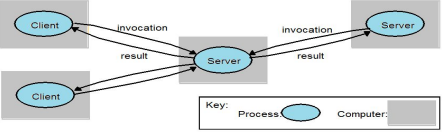
\includegraphics[scale=1.2]{3.png}
\end{frame}


\begin{frame}{A typical distributed application based on peer processes}
	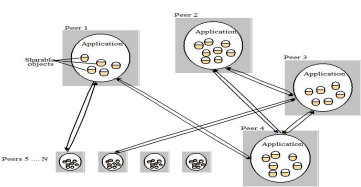
\includegraphics[scale=1.4]{4.png}
\end{frame}


\section{\textbf{Grid Computing}}

\begin{frame}{Grid Computing?}
	\begin{itemize}
		\item Pcwebopedia.com \\
		 – A form of networking. unlike conventional networks that focus on communication 
		among devices, grid computing harnesses unused processing cycles of all computers in 
		a network for solving problems too intensive for any stand-alone machine.
		
		\item IBM \\
		– Grid computing enables the virtualization of distributed computing and data resources 
		such as processing, network bandwidth and storage capacity to create a single system 
		image, granting users and applications seamless access to vast IT capabilities. Just as 
		an Internet user views a unified instance of content via the Web, a grid user essentially 
		sees a single, large virtual computer.
		
		
		\item Sun Microsystems \\
		
		– Grid Computing is a computing infrastructure that provides dependable, 
		consistent, pervasive and inexpensive access to computational capabilities
		
		
		
	\end{itemize}
\end{frame}


\begin{frame}{Grid Computing}
	\begin{enumerate}
		
		\item  Share more than information: Data, computing power, applications in 
		dynamic environment, multi-institutional, virtual organizations \\
		\item  Efficient use of resources at many institutes. People from many institutions
		working to solve a common problem (virtual organisation). \\
		\item  Join local communities. \\
		\item  Interactions with the underneath layers must be transparent and seamless 
		to the user.
		
	\end{enumerate}
\end{frame}


\begin{frame}{ Need Of Grid Computing?}
	\begin{itemize}
		
		\item   Today’s Science/Research is based on computations, data analysis, data 
		visualization & collaborations
		\item Computer Simulations & Modelling are more cost effectivethan
		experimental methods
		\item  JScientific and Engineering problems are becoming more complex & users 
		need more accurate, precise solutions to their problems in shortest possible 
		time
		\item  Data Visualization is becoming very important
		\item Exploiting under utilized resources
		
	\end{itemize}
\end{frame}



\begin{frame}{Who uses Grid Computing ?}
	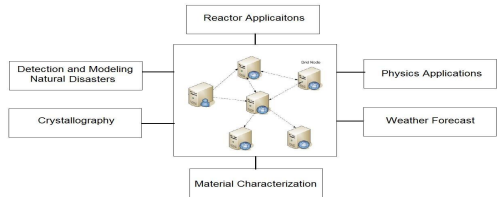
\includegraphics[scale=1.0]{5.png}
\end{frame}

\begin{frame}{ Types Of Grids}
	\begin{itemize}
		
		\item  \textbf{Computational Grid:} These grids provide secure access to huge pool of shared processing 
		power suitable for high throughput applications and computation intensive computing.
		\item \textbf{Data Grid:} Data grids provide an infrastructure to support data storage, data discovery, data 
		handling, data publication, and data manipulation of large volumes of data actually stored 
		in various heterogeneous databases and file systems.
		\item  \textbf{Collaboration Grid:} With the advent of Internet, there has been an increased demand for 
		better collaboration. Such advanced collaboration is possible using the grid. For instance, 
		persons from different companies in a virtual enterprise can work on different components of 
		a CAD project without even disclosing their proprietary technologies
		
	\end{itemize}
\end{frame}

\begin{frame}{}
	\begin{itemize}
		
		\item \textbf{Network Grid:} A Network Grid provides fault-tolerant and high-performance communication 
		services. Each grid node works as a data router between two communication points, 
		providing data-caching and other facilities to speed up the communications between such 
		points.
		
		\item  \textbf{Utility Grid:} This is the ultimate form of the Grid, in which not only data and computation 
		cycles are shared but software or just about any resource is shared. The main services 
		provided through utility grids are software and special equipment. For instance, the 
		applications can be run on one machine and all the users can send their data to be 
		processed to that machine and receive the result back
		
	\end{itemize}
\end{frame}

\begin{frame}{Grid Components}
	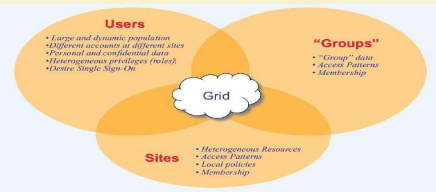
\includegraphics[scale=1.2]{6.png}
\end{frame}


\section{\textbf{Cluster Computing}}



\begin{frame}{What is Cluster Computing?}
	\begin{itemize}
		
		\item   A cluster is a type of parallelor distributed
		computer system, which consists of a
		collection of inter-connected stand-alone computers 
		working together as a single integrated
		computing resource .
		\item Key components of a cluster include multiple 
		standalone computers (PCs, Workstations, or SMPs), 
		operating systems, high-performance interconnects, 
		middleware, parallel programming environments, and
		applications.
		
	\end{itemize}
\end{frame}

\begin{frame}{ Cluster Computing}
	\begin{itemize}
		
		\item   Clusters are usually deployed to improve speed and/or reliability 
		over that provided by a single computer, while typically being 
		much more cost effective than single computer the of comparable 
		speed or reliability
		\item In a typical cluster \\ \\
		– Network: Faster, closer connection than a typical 
		network (LAN) \\
		– Low latency communication protocols \\
		– Loosely coupled than SMP
		
		
		
		
	\end{itemize}
\end{frame}


\begin{frame}{Types of Cluster}
	\begin{itemize}
		
		\item High Availability or Failover Clusters
		\item Load Balancing Cluster
		\item Parallel/Distributed Processing 
		Clusters
		
		
	\end{itemize}
\end{frame}


\begin{frame}{Cluster Components}
	\begin{itemize}
		
		\item Basic building blocks of clusters are broken down into 
		multiple categories :
		\item \textbf{Cluster Nodes}
		\item \textbf{Cluster Network}
		\item \textbf{Network Characterization}
		
			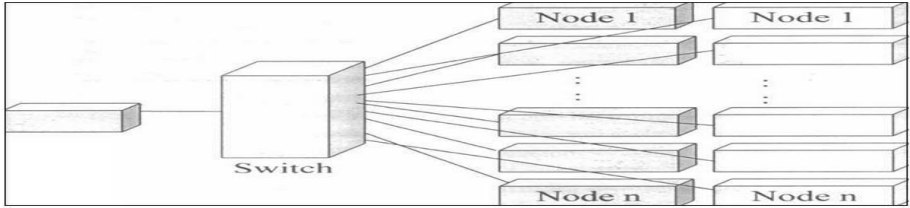
\includegraphics[scale=0.5]{7.png}
		
		
	\end{itemize}
\end{frame}


\begin{frame}{Key Operational Benefits of Clustering}
	\begin{itemize}
		
		\item   System availability: offer inherent high system availability due to the redundancy of hardware, operating systems, and applications.
		\item Hardware fault tolerance: redundancy for most system 
		components (eg. disk-RAID), including both hardware and 
		software.
		\item OS and application reliability: run multiple copies of the OS	and applications, and through this redundancy
		\item Scalability. adding servers to the cluster or by adding more clusters to the network as the need arises or CPU to SMP.
		
	\end{itemize}
\end{frame}

\section{\textbf{Utility Computing}}

\begin{frame}{“Utility” Computing?}
	\begin{itemize}
		
		\item Utility Computing is purely a concept which cloud computing practically implements.
		\item Utility computing is a service provisioning model in which a service provider makes 
		computing resources and infrastructure management available to the customer as 
		needed, and charges them for specific usage rather than a flat rate.
		\item This model has the advantage of a low or no initial cost to acquire computer resources; 
		instead, computational resources are essentially rented.
		\item The word utility is used to make an analogy to other services, such as electrical power, 
		that seek to meet fluctuating customer needs, and charge for the resources based on 
		usage rather than on a flat-rate basis. This approach, sometimes known as pay-per-use
		
		
	\end{itemize}
\end{frame}



\begin{frame}{Utility Computing Example}
	\begin{itemize}
		
		\item On-Demand Cyber
		\item Infrastructure
		
			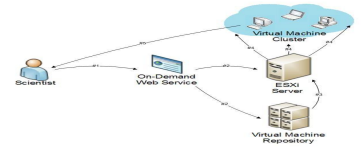
\includegraphics[scale=1.5]{9.png}
		
		
		
	\end{itemize}
\end{frame}

\begin{frame}{Utility Solution – Your 
		Perspective Consumer Provider}
	
		
		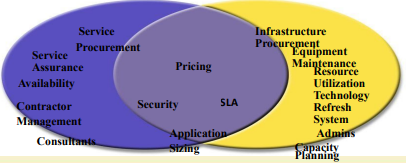
\includegraphics[scale=1.5]{10.png}
		
		
		

\end{frame}



\begin{frame}{ Utility Computing Payment Models}
	\begin{itemize}
		
		\item   Same range of charging models as other utility providers: gas, electricity, telecommunications, water, 
		television broadcasting \\
		 - Flat rate \\
		 - Tiered \\
		 - Subscription \\
		 - Metered \\
		 - Pay as you go \\
		 - Standing charges \\
		\item Different pricing models for different customers based on factors such as scale, commitment and 
		payment frequency
		\item But the principle of utility computing remains
		\item The pricing model is simply an expression by the provider of the costs of provision of the resources and a 
		profit margin
		
	\end{itemize}
\end{frame}

%% RIYA'S CODE

\begin{frame}{ Risks in a UC World}
	\begin{itemize}
		
		\item  Data Backup
		\item Data Security
		\item Partner Competency
		\item Defining SLA
		\item Getting value from charge back
		
	\end{itemize}
\end{frame}


\section{\textbf{Cloud Computing}}

\begin{frame}{Cloud Computing}
	\begin{itemize}
		\item US National Institute of Standards and Technology defines Computing as:
		\item Cloud computing is a model for enabling ubiquitous, convenient, on-demand network access to a shared pool of 
		configurable computing resources (e.g networks, servers, storage, applications, and services) that can be 
		rapidly provisioned and released with minimal management effort or service provider interaction. ”
		
		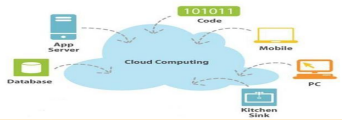
\includegraphics[scale=1.5]{11.png}
		
	\end{itemize}
\end{frame}

\section{\textbf{Thank You!!}}

\begin{frame}
	\titlepage
\end{frame}

\section{\textbf{Cloud Computing}}



\begin{frame}{Cloud Computing}
	\begin{itemize}
	\item US \textbf{National Institute of Standards and Technology (NIST)} defines Computing as:
		\item Cloud computing is a model for enabling ubiquitous, convenient, on-demand network access to a shared pool of 
		configurable computing resources (e.g networks, servers, storage, applications, and services) that can be 
		rapidly provisioned and released with minimal management effort or service provider interaction. ”
		
		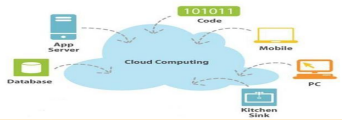
\includegraphics[scale=1.5]{11.png}
		
	\end{itemize}
\end{frame}


\begin{frame}{ Essential Characteristics}
	\begin{itemize}
		
		\item  \textbf{On-demand self-service}
		        	\begin{itemize}
		        	
		        	\item A consumer can unilaterally provision computing capabilities, such as server time and network storage, as 
		        	needed automatically without requiring human interaction with each service provider.
		        	
		        \end{itemize}
		\item \textbf{Broad network access}
		        \begin{itemize}
		        	
		        	\item Capabilities are available over the network and accessed through standard mechanisms that promote use by 
		        	heterogeneous thin or thick client platforms (e.g., mobile phones, tablets, laptops, and workstations).
		        \end{itemize}
		\item \textbf{Resource pooling}
		          \begin{itemize}
		          	
		          	\item The provider’s computing resources are pooled to serve multiple consumers using a multi-tenant model, 
		          	with different physical and virtual resources dynamically assigned and reassigned according to consumer 
		          	demand.
		          	
		          \end{itemize}
	\end{itemize}
\end{frame}


\begin{frame}{ Cloud Characteristics}
	\begin{itemize}
		
		\item  \textbf{Measured Service}
		\begin{itemize}
			\item Cloud systems automatically control and optimize resource use by leveraging a metering 
			capability at some level of abstraction appropriate to the type of service (e.g., storage, 
			processing, bandwidth, and active user accounts). Resource usage can be
			\item monitored, controlled, and reported, providing transparency for both the provider and 
			consumer of the utilized service.
			
		\end{itemize}
		\item \textbf{Rapid elasticity}
		\begin{itemize}
			
			\item Capabilities can be elastically provisioned and released, in some cases automatically, 
			to scale rapidly outward and inward commensurate with demand. To the consumer, 
			the capabilities available for provisioning often appear to be unlimited and can be appropriated in any quantity at any time.
		\end{itemize}
	\end{itemize}
\end{frame}


\begin{frame}{ Common Characteristics}
	\begin{itemize}
		
		\item Massive Scale
		\item Resilient Computing Homogeneity
		\item Geographic Distribution
		\item Virtualization
		\item Service Orientation
		\item Low Cost Software
		\item Advanced Security
		
		
	\end{itemize}
\end{frame}


\begin{frame}{Cloud Services Models}
	\begin{itemize}
		
		\item  \textbf{Software as a Service (SaaS)}
		\begin{itemize}
			
			\item The capability provided to the consumer is to use the provider’s applications running on a cloud infrastructure. The applications 
			are accessible from various client devices through either a thin client interface, such as a web browser (e.g., web-based email), or 
			a program interface.
			
			\item The consumer does not manage or control the underlying cloud infrastructure including network, servers, operating systems, 
			storage, or even individual application capabilities, with the possible exception of limited user-specific application configuration 
			settings.
			
			\item e.g: Google Spread Sheet
			
		\end{itemize}
		\item \textbf{Cloud Infrastructure as a Service (IaaS)}
		\begin{itemize}
			
			\item The capability provided to provision processing, storage, networks, and other fundamental computing resources
			\item Consumer can deploy and run arbitrary software
			\item e.g: Amazon Web Services and Flexi scale.
		\end{itemize}
	\end{itemize}
\end{frame}


\begin{frame}{Cloud Services Models}
	\begin{itemize}
		
		\item  \textbf{Platform as a Service (PaaS)}
		\begin{itemize}
			
			\item The capability provided to the consumer is to deploy onto the cloud infrastructure consumer-created or 
			acquired applications created using programming languages, libraries, services, and tools supported by the 
			provider.
			
			\item The consumer does not manage or control the underlying cloud infrastructure including network, servers, 
			operating systems, or storage, but has control over the deployed applications and possibly configuration 
			settings for the application-hosting environment.
			
		\end{itemize}
	\end{itemize}
\end{frame}

\begin{frame}{Cloud Services Models}
    
     	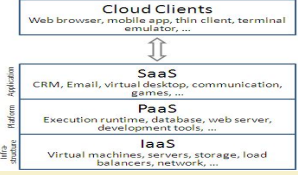
\includegraphics[scale=1.5]{12.png}
     
\end{frame}



\begin{frame}{Types of Cloud (Deployment Models)}
	\begin{itemize}
		
	\item  \textbf{Private Cloud} \\
	The cloud infrastructure is operated solely for an organization.
	e.g Window Server 'Hyper-V'. \\
	
	\item  \textbf{Community Cloud} \\
	The cloud infrastructure is shared by several organizations and supports a specific goal.
	
	\item \textbf{Public cloud} \\
	The cloud infrastructure is made available to the general public
	e.g Google Doc, Spreadsheet.
	\item \textbf{Hybrid Cloud} \\
	The cloud infrastructure is a composition of two or more clouds (private, community, or public)
	e.g Cloud Bursting for load balancing between clouds.
	
	\end{itemize}
\end{frame}

\begin{frame}{Cloud and Virtualization}
	\begin{itemize}
		
		\item  \textbf{Virtual Workspaces:} 
		\begin{itemize}
			\item An abstraction of an execution environment that can be made dynamically available to
			authorized clients by using well-defined protocols,
			\item Resource quota (e.g. CPU, memory share),
			\item Software configuration (e.g. OS)
			
		\end{itemize}
	     \item  \textbf{Implement on Virtual Machines (VMs):} 
	     \begin{itemize}
	     	\item  Abstraction of a physical host machine
	     	\item Hypervisor intercepts and emulates instructions from VMs, and allows management of VMs
	     	\item VMWare, Xen, KVM etc.
	     	
	     \end{itemize}
	     \item  \textbf{Provide infrastructure API:} 
	     \begin{itemize}
	     	\item  Plug-ins to hardware/support 
	     	structures 
	     \end{itemize}
	     
	\end{itemize}
	
	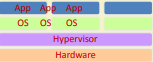
\includegraphics[scale=1.5]{13.png}
	
\end{frame}


\begin{frame}{Cloud and Virtualization}
	\begin{itemize}
		
		\item  VM technology allows multiple virtual machines to run on a single
		physical machine.
		
		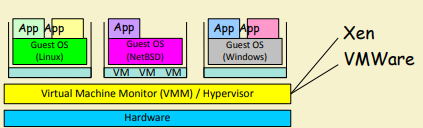
\includegraphics[scale=1.2]{14.png}
		
		\item Performance: Para-virtualization (e.g. Xen) is very close to raw physical
		performance!
	\end{itemize}
\end{frame}


\begin{frame}{Virtualization in General}
	\begin{itemize}
		
		\item  \textbf{Advantages of virtual machines:}
		\begin{itemize}
			\item  Run operating systems where the physical hardware is unavailable,
			\item  Easier to create new machines, backup machines, etc.,
			\item Software testing using “clean” installs of operating systems and software,
			\item  Emulate more machines than are physically available,
			\item  Timeshare lightly loaded systems on one host,
			\item  Debug problems (suspend and resume the problem machine),
			\item  Easy migration of virtual machines (shutdown needed or not).
			\item  Run legacy systems
			
			
		\end{itemize}
	\end{itemize}
\end{frame}


\begin{frame}{Cloud-Sourcing}
	\begin{itemize}
		
		\item  \textbf{Why is it becoming important ?}
		\begin{itemize}
			\item  Using high-scale/low-cost providers,
			\item  Any time/place access via web browser,
			\item  Rapid scalability; incremental cost and load sharing,
			\item  Can forget need to focus on local IT.
		\end{itemize}
		\item  \textbf{Concerns:}
		\begin{itemize}
		\item  Performance, reliability, and SLAs,
		\item  Control of data, and service parameters,
		\item  Application features and choices,
		–\item Interaction between Cloud providers,
		\item  No standard API – mix of SOAP and REST!
		\item  Privacy, security, compliance, trust…
		
		\end{itemize}
	\end{itemize}
\end{frame}



\begin{frame}{Cloud-Storage}
	\begin{itemize}
		
		\item  Several large Web companies are now exploiting the fact that they have data
		storage capacity that can be hired out to others.
		\begin{itemize}
			\item  Allows data stored remotely to be temporarily cached on 
			desktop computers, mobile phones or other 
			Internet-linked devices.
		\end{itemize}
		\item  Amazon’s Elastic Compute Cloud (EC2) and Simple Storage Solution (S3) are well
		known examples
	\end{itemize}
\end{frame}

\begin{frame}{Advantages of Cloud Computing}
	\begin{itemize}
		
		\item  \textbf{Lower computer costs:}
		\begin{itemize}
			\item  No need of a high-powered and high-priced computer to run cloud computing's 
			web-based applications.
			\item  Since applications run in the cloud, not on the desktop PC, your desktop PC does not 
			need the processing power or hard disk space demanded by traditional desktop 
			software.
			\item  When you are using web-based applications, your PC can be less expensive, with a
			smaller hard disk, less memory, more efficient processor...
			\item  In fact, your PC in this scenario does not even need a CD or DVD drive, as no 
			software programs have to be loaded and no document files need to be saved.
			
		\end{itemize}
		
	\end{itemize}
\end{frame}
\begin{frame}{Advantages of Cloud Computing}
	\begin{itemize}
		
		\item  \textbf{Improved performance:}
		\begin{itemize}
			\item  With few large programs hogging your computer's memory, you will see better 
			performance from your PC.
			\item  Computers in a cloud computing system boot and run faster because they have 
			fewer programs and processes loaded into memory.
			
		\end{itemize}
			\item  \textbf{Reduced software costs:}
		\begin{itemize}
			\item  Instead of purchasing expensive software applications, you can get most of what 
			you need for free. \\
			• most cloud computing applications today, such as the Google Docs suite.
			\item  better than paying for similar commercial software \\
			• which alone may be justification for switching to cloud applications.
			
			
		\end{itemize}
	\end{itemize}
\end{frame}

\begin{frame}{Advantages of Cloud Computing}
	\begin{itemize}
		
		\item  \textbf{Instant software updates}
		\begin{itemize}
			\item  Another advantage to cloud computing is that you are no longer faced with choosing
			between obsolete software and high upgrade costs.
			\item  When the application is web-based, updates happen automatically available the next time 
			you log into the cloud.
			\item  When you access a web-based application, you get the latest version without needing to pay 
			for or download an upgrade.
			
		\end{itemize}
		\item  \textbf{Improved document format compatibility.}
		\begin{itemize}
			\item  You do not have to worry about the documents you create on your machine being 
			compatible with other users' applications or OS.
			\item  There are less format incompatibilities when everyone is sharing documents and 
			applications in the cloud.
			
		\end{itemize}
	\end{itemize}
\end{frame}






\begin{frame}{Advantages of Cloud Computing}
	\begin{itemize}
		
		\item  \textbf{Unlimited storage capacity}
		\begin{itemize}
		\item  Cloud computing offers virtually limitless storage.
		\item  Your computer's current 1 Tera Bytes hard drive is small compared to the hundreds of Peta 
		Bytes available in the cloud.
			
		\end{itemize}
		\item  \textbf{Increased data reliability}
		\begin{itemize}
		\item  Unlike desktop computing, in which if a hard disk crashes and destroy all your 
		valuable data, a computer crashing in the cloud should not affect the storage of your 
		data. \\
		• if your personal computer crashes, all your data is still out there in the cloud, still accessible
		\item  In a world where few individual desktop PC users back up their data on a regular basis, 
		cloud computing is a data-safe computing platform. For e.g. Dropbox, Skydrive
		
		\end{itemize}
	\end{itemize}
\end{frame}

\begin{frame}{Advantages of Cloud Computing}
	\begin{itemize}
		
		\item  \textbf{Universal information access}
		\begin{itemize}
			\item  That is not a problem with cloud computing, because you do not take your
			documents with you.
			\item  Instead, they stay in the cloud, and you can access them whenever you have a 
			computer and an Internet connection
			\item  Documents are instantly available from wherever you are.
			
		\end{itemize}
		\item  \textbf{Latest version availability}
		\begin{itemize}
			\item  When you edit a document at home, that edited version is what you see when
			you access the document at work.
			\item  The cloud always hosts the latest version of your documents as long as you are 
			connected, you are not in danger of having an outdated version
			
		\end{itemize}
	\end{itemize}
\end{frame}


\begin{frame}{Advantages of Cloud Computing}
	\begin{itemize}
		
		\item  \textbf{Easier group collaboration}
		\begin{itemize}
			\item  Sharing documents leads directly to better collaboration.
			\item  Many users do this as it is an important advantages of cloud computing
			multiple users can collaborate easily on documents and projects
			
		\end{itemize}
		\item  \textbf{Device independence}
		\begin{itemize}
			\item  You are no longer tethered to a single computer or network.
			\item  Changes to computers, applications and documents follow you through the
			cloud.
			\item  Move to a portable device, and your applications and documents are still 
			available
			
		\end{itemize}
	\end{itemize}
\end{frame}

\begin{frame}{Disadvantages of Cloud Computing}
	\begin{itemize}
		
		\item  \textbf{Requires a constant internet connection}
		\begin{itemize}
		\item  Cloud computing is impossible if you cannot connect to the Internet.
		\item  Since you use the Internet to connect to both your applications and documents, if you do not 
		have an Internet connection you cannot access anything, even your own documents.
		\item  A dead Internet connection means no work and in areas where Internet connections are few or 
		inherently unreliable, this could be a deal-breaker
			
		\end{itemize}
		\item  \textbf{Does not work well with low-speed connections}
		\begin{itemize}
			\item  Similarly, a low-speed Internet connection, such as that found with dial-up services, makes 
			cloud computing painful at best and often impossible.
			\item  Web-based applications require a lot of bandwidth to download, as do large documents
			
		\end{itemize}
	\end{itemize}
\end{frame}



\begin{frame}{Disadvantages of Cloud Computing}
	\begin{itemize}
		
		\item  \textbf{Features might be limited}
		\begin{itemize}
			\item  This situation is bound to change, but today many web-based applications simply 
			are not as full-featured as their desktop-based applications. \\
			• For example, you can do a lot more with Microsoft PowerPoint than with Google 
			Presentation's web-based offering
			
		\end{itemize}
		\item  \textbf{ Can be slow}
		\begin{itemize}
			\item Even with a fast connection, web-based applications can sometimes be slower than 
			accessing a similar software program on your desktop PC.
			\item  Everything about the program, from the interface to the current document, has to
			be sent back and forth from your computer to the computers in the cloud.
			\item  If the cloud servers happen to be backed up at that moment, or if the Internet is 
			having a slow day, you would not get the instantaneous access you might expect 
			from desktop applications.
			
		\end{itemize}
	\end{itemize}
\end{frame}


\begin{frame}{Disadvantages of Cloud Computing}
	\begin{itemize}
		
		\item  \textbf{Stored data might not be secured}
		\begin{itemize}
		\item  With cloud computing, all your data is stored on the cloud. \\
		• The questions is How secure is the cloud?
		\item  Can unauthorized users gain access to your confidential data ?
			
		\end{itemize}
		\item  \textbf{Stored data can be lost!}
		\begin{itemize}
			\item  Theoretically, data stored in the cloud is safe, replicated across multiple machines.
			\item  But on the off chance that your data goes missing, you have no physical or local backup. \\
			• Put simply, relying on the cloud puts you at risk if the cloud lets you down.
			
			
		\end{itemize}
	\end{itemize}
\end{frame}

\begin{frame}{Disadvantages of Cloud Computing}
	\begin{itemize}
		
		\item  \textbf{HPC Systems}
		\begin{itemize}
		\item  Not clear that you can run compute-intensive HPC applications that use MPI/OpenMP!
		\item  Scheduling is important with this type of application \\
		• as you want all the VM to be co-located to minimize communication latency!
			
		\end{itemize}
		\item  \textbf{General Concerns}
		\begin{itemize}
		\item  Each cloud systems uses different protocols and different APIs \\
		• may not be possible to run applications between cloud based systems
		\item  Amazon has created its own DB system (not SQL 92), and workflow system (many 
		popular workflow systems out there)\\
		• so your normal applications will have to be adapted to execute on these platforms.
			
			
		\end{itemize}
	\end{itemize}
\end{frame}

%% RIYA'S CODE ENDS



\end{document}
